\section{Optimal Dynamic Portfolio}

While the static portfolios are valuable to understand the tradeoffs between the various NET's in regards to cost and speed of deployment, they are of limited use in providing policy recommendations for the goal set in the Paris agreement of limiting global warming to below 2 °C. In order to achieve this goal, the UN Environment Programme has estimated CDR targets of 3.8 Gt annually by 2035, increasing to 9.2 Gt by 2050 and 20 Gt by 2100 \parencite{unep_emissions_2023}. In order to appropriately reflect these targets, a dynamic optimization approach, which considers the need to continually remove an ever-increasing amount of CO$_2$, is required.\vspace{2mm}

The dynamic portfolio was developed from the same fundamental constraints applied to the static optimization. The primary difference is that instead of a fixed amount of CO$_2$ to be removed over a set timeframe, a segmented, linearly increasing function was used, starting from zero in the year 2026 and ramping up in three segments to reach the above-mentioned CDR targets. Additionally, due to the dynamic nature of the model, the costs of each NET over the entire time frame were discounted to the year 2026 at a discount rate of $r = 7\%$.\vspace{2mm}

\subsection{Model Formulation}
\subsubsection{Objective function}
In the dynamic optimization model, the time period $ T =  \{0,1,...,T\} $ is defined, where $t=0$ corresponds to the start year $y_0 = 2026$, and $t=T$ to the final year $y_T = 2101$, creating a 75 year modeling horizon. Smiliar to the static model, the dynamic model determines the least-cost portfolio of afforestation, BECCS, enhanced weathering, and direct air capture. However, the removal target $R$ is not defined as one cumulative amount, but rather an annual removal trajectory, generated by linear interpolation between the targets $R_{5} = 2500$, $R_{10} = 3800$, $R_{25} = 9200$, $R_{75} = 20000$. Additionally, the dynamic model uses discounted cost values to properly account for the time value of money. The value of carbon removed is not discounted, since atmospheric carbon is considered to have the same effect irrespective of time.\vspace{2mm}

The optimization problem can thus be written as
\begin{equation}
  \text{min} \sum \delta_t \left[ K^{\text{A/R}}_t + K^{\text{BECCS}}_t + K^{\text{ERW}}_t + K^{\text{DAC}}_t \right]
\end{equation}
where $\delta_t = \frac{1}{(1+r)^t}$ and $r=0.07.$

\subsubsection{Afforestation/Reforestation}
The A/R model is modified to include an annual reversal risk of 1\%. Let $\alpha^\text{A/R} = 0.01$ denote the annual reversal rate. Then the forest stock evolves as
\begin{equation}
X_{t,c}^\text{A/R} =
    \begin{cases}
      x_{t,c}^\text{A/R}, & t = 0,\\
      (1-\alpha^\text{A/R})X_{t-1,c}^\text{A/R}+x_{t,c}^\text{A/R} & t > 0,
    \end{cases}
    \qquad \forall c \in \mathcal{C}
\end{equation}
The land-availability and annual-expansion constraints remain as in the static model, but the annual A/R removals are adjusted for survival so that
\begin{equation}
q^{\text{A/R}}_t = 
    \begin{cases}
      0, & t = 0,\\
      \sum_{c\in \mathcal{C}}\sum_{\tau=\text{max}(0,t-g_c)}^{t-1} \alpha_cx_{\tau,c}^\text{A/R}(1-\rho^\text{A/R})^{t-\tau} & t > 0,
    \end{cases} 
\end{equation}

\subsubsection{BECCS}
Compared to the static model, the BECCS implementation in the dynamic model uses capacity expansion and operation as separate decision variables, similar to the DAC model.\vspace{2mm}

Let $\mathcal{C}^\text{BECCS}$ be the set of countries with BECCS potential, and $\mathcal{B}$ the set of biomass types available. Then, $\mathcal{P}\subseteq\mathcal{C}^\text{BECCS}\times\mathcal{B}$ is the set of country-biomass pairs available. For each $(c,b) \in \mathcal{P}$, let $a_{c,b}$ be the constant amount of biomass available per country, $\eta_{c,b}^{cap}$ the captured CO$_2$ per unit of biomass, $\eta_{c,b}^{pow}$ the electricity exported per unit of biomass, $k_{c,b}^{bm}$ the cost per unit of biomass, and $k_{c,b}^{var}$ and $k_{c,b}^{ts}$ the variable cost and transport and storage cost, respectively, per captured unit of CO$_2$.\vspace{2mm}

The installed BECCS capacity evolves analogously to the DAC model, as
\begin{equation}
X_{t,c}^\text{BECCS} =
    \begin{cases}
      x_{t,c}^\text{BECCS}, & t = 0,\\
      \sum^{t-1}_{\tau=\text{max}(0,t-L^\text{BECCS})} x_{t,c}^\text{BECCS} & t > 0,
    \end{cases}
    \qquad \forall c \in \mathcal{C}^{BECCS}
\end{equation}
where $L^\text{BECCS}$ is the assumed plant lifetime, which is also set at 20 years. The capacity expansion is again subject to an initial build limit and an annual growth constraint proportionate to the previous years' capacity, denoted in MW gross electricity generation:
\begin{equation}
x_{t,c}^\text{BECCS} \leq
    \begin{cases}
      1000, & t = 0,\\
      \phi^{\text{BECCS}}X_{t-1,c}^{\text{BECCS}} & t > 0,
    \end{cases}
    \qquad \forall k \in \mathcal{C}^\text{BECCS}
\end{equation}
while the biomass use is limited by the resource availability:
\begin{equation}
u_{t,c,b}^\text{bm} \leq a_{c,b}^\text{bm} \qquad \forall t \in T, (c,b) \in \mathcal{P}.
\end{equation}
Gross carbon captured is then proportional to the biomass throughput:
\begin{equation}
q_{t,c,b}^\text{gross} = \eta_{c,b}^{cap}u_{t,c,b}^{bm} \qquad \forall t \in T, (c,b) \in \mathcal{P}.
\end{equation}
The installed BECCS power capacity limits the annual biomass throughput through an energy-output constraint:
\begin{equation}
\sum_{b\in \mathcal{B}(c)} u_{t,c,b}^{bm}\eta_{c,b}^{pow} \leq X_{t,c}^\text{BECCS}h^\text{FLH}\gamma^{CF}(1-\ell^{aux})  \qquad \forall t \in T, c \in \mathcal{C}^\text{BECCS}
\end{equation}
where $\mathcal{B}(c)$ denotes the set of biomass types availabile in country $c$, $h^\text{FLH}$ the full-load hours, $\gamma^\text{CF}$ the average capacity factor, and $\ell^{aux}$ the auxiliary energy loss.\vspace{2mm}

The net BECCS carbon removal per year are finally computed as the amount of CO$_2$ net of the leakage:
\begin{equation}
q_{t}^\text{BECCS} = (1-\alpha^\text{BECCS}) \sum_{(c,b)\in \mathcal{P}}q_{t,c,b}^\text{gross} \qquad \forall t \in T.
\end{equation}
where $\alpha^\text{BECCS}$ is the BECCS leakage factor.\vspace{2mm}

The annual costs of BECCS are then calculated as the sum of capital expenditures, fixed operating costs, and variable costs, less revenue from electricity export. Specifically,
\begin{equation}
K_t^\text{BECCS,CapEx} = \sum_{c \in \mathcal{C}^\text{BECCS}} I^\text{BECCS}x_{t,c}^\text{BECCS},
\end{equation}
\begin{equation}
K_t^\text{BECCS,fixed} = \sum_{c \in \mathcal{C}^\text{BECCS}} k^\text{BECCS,fixed}X_{t,c}^\text{BECCS},
\end{equation}
\begin{equation}
K_t^\text{BECCS,var} = \sum_{(c,b) \in \mathcal{P}} \left[ k_{c,b}^{bm}u_{t,c,b}^{bm} + \left( k_{c,b}^\text{var} + k_{c,b}^{ts} \right) q_{t,c,b}^\text{gross} \right],
\end{equation}
with electricity revenue
\begin{equation}
Rev_t^\text{BECCS,pow} = \sum_{c \in \mathcal{C}^\text{BECCS}} X_{t,c}^\text{BECCS}h^\text{FLH}\gamma^\text{CF}(1-\ell^\text{aux})p_c^\text{pow}.
\end{equation}
Note that the fixed cost is calculated based on the total installed capacity, irrespective of actual operation, while variable cost is based on the amount of biomass consumed and the additional variable costs per unit of CO$_2$ captured. The total BECCS cost in year $t$ is then

\begin{equation}
K_t^{\text{BECCS}} = K_t^{\text{BECCS,CapEx}} + K_t^{\text{BECCS,fixed}} + K_t^{\text{BECCS,var}}- Rev_t^{\text{BECCS,pow}}.
\end{equation}

\subsection{Results}

\begin{figure}[ht!]
  \begin{center}
    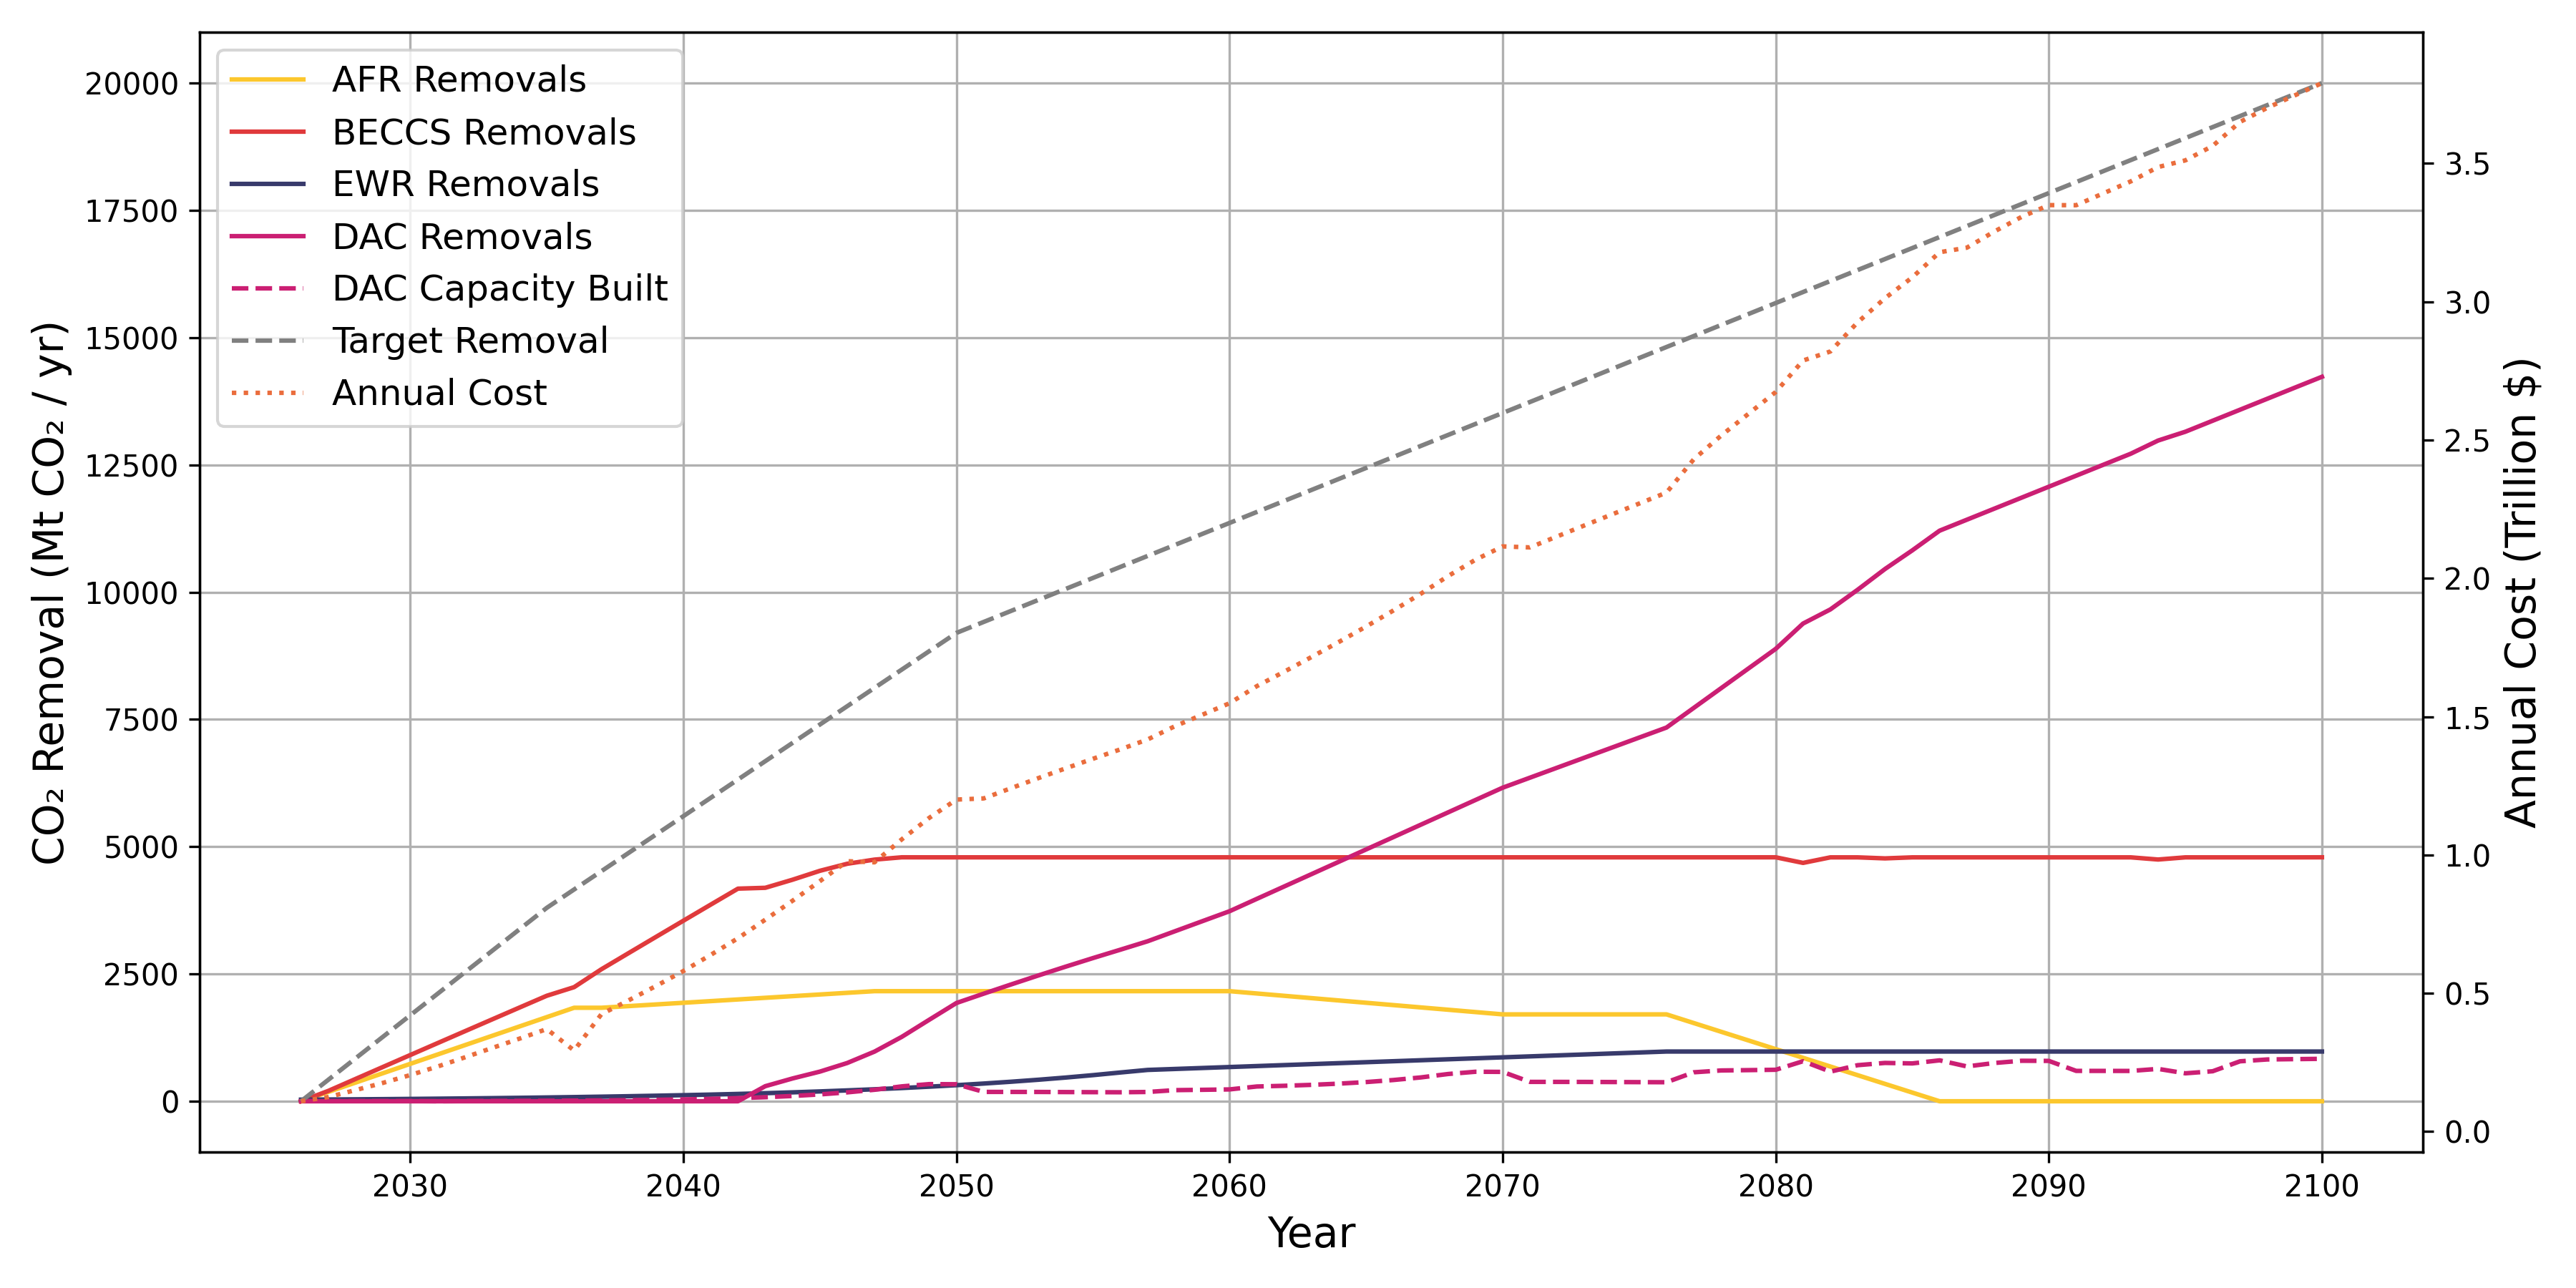
\includegraphics[width=1\linewidth]{figures/optimal_dynamic_portfolio.png}
    \caption{Optimal dynamic portfolio (up to year 2100)}
    \label{fig:optimal_dynamic_portfolio}
  \end{center}
  \vspace*{-\baselineskip}
\end{figure}

The resulting portfolio is shown in figure 4.3. The A/R approach is immediately deployed to its maximum potential, and constrained only by the annual expansion limit and the overall available land area. Additionally, BECCS is also immediately deployed to cover the remaining CDR gap that A/R cannot fulfill, and is ramped up until it reaches its maximum as constrained by the available waste biomass. For DAC, investment and construction begins immediately, but its operation only begins once A/R and BECCS are near their maximum. It later carries the bulk of the CDR efforts from the mid 2060s onwards. Enhanced Weathering is also deployed from the get go, but only plays a very limited role, due to the likely logistical and bureaucratic limitations considered in the model. In total, this portfolio includes 855 Gt of CDR between 2026 and 2100, at a cost of 136 trillion US\$.\vspace{2mm}

\begin{table}[]
\renewcommand{\arraystretch}{1.4}
\begin{tabular}{lrrr}
Technology     & \multicolumn{1}{l}{Amount removed (Mt)} & \multicolumn{1}{l}{Total cost (B US\$)} & \multicolumn{1}{l}{Average LCOC (US\$)} \\ \hline
\textbf{A/R}   & 97,250                                  & 1,809                                  & 18.60                                  \\
\textbf{ERW}   & 45,177                                  & 1,257                                  & 27.82                                  \\
\textbf{BiCRS} & 309,081                                 & 46,407                                 & 150.15                                 \\
\textbf{DAC}   & 403,123                                 & 86,623                                 & 214.88                                 \\ \hline
\textbf{Total} & 854,631                                 & 136,096                                & 159,25                                 \\ \hline
\end{tabular}
\captionof{table}{Breakdown of amounts removed and cost by NET}
\end{table}

Looking at the development of the levelized cost per tonne of CO$_2$ for the different NET's over the timeline until the year 2100 in figure 4.4, a few curious observations can be made. First, the cost of ERW stays nearly constant. This is largely due to the modeling constraints, which limit the actual deployment of the technology to a point significantly below the hypothetical potential shown by the MACC developed in chapter 3.3. Second, The LCOC's of A/R, and to a more significant degree, of BiCRS, are actually increasing over time. This is because the optimizer uses the cheapest potential first, and once this is exhausted, moves to add the more expensive options. Third, the LCOC of DAC seems to decrease only by little, dropping from 225 in 2043 to 212 by 2100. \vspace{2mm}

\begin{figure}[ht!]
  \begin{center}
    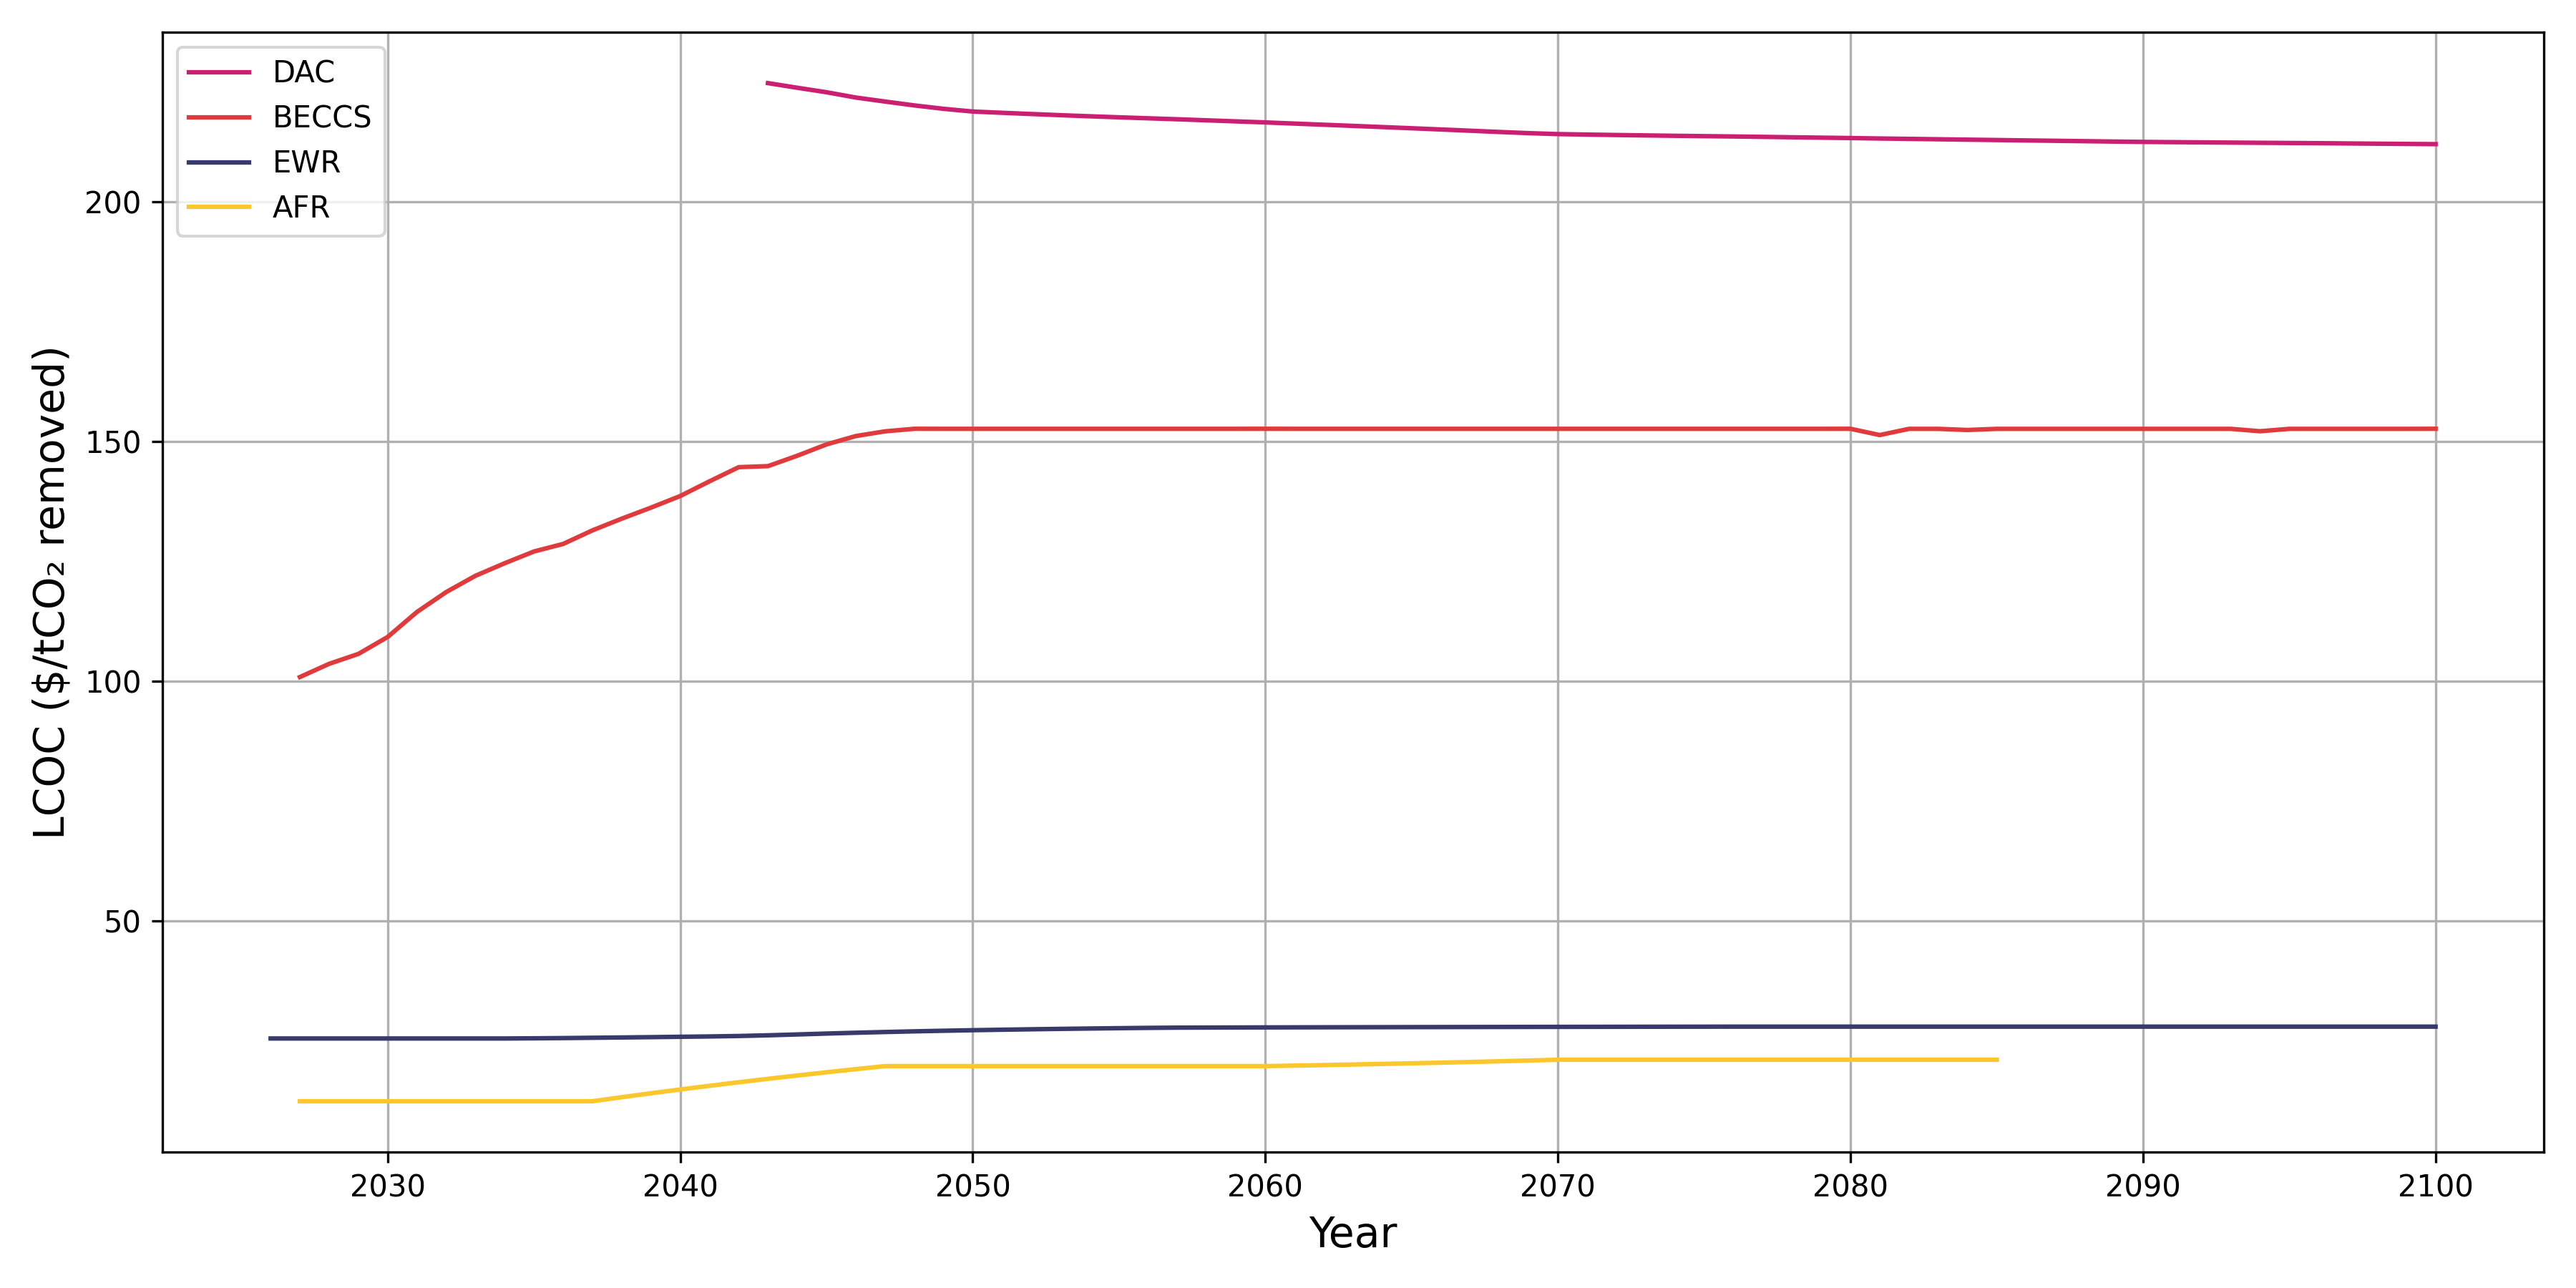
\includegraphics[width=1\linewidth]{figures/annual_lcoc_by_tech.png}
    \caption{Development of LCOC's by NET}
    \label{fig:annual_lcoc_by_tech}
  \end{center}
  \vspace*{-\baselineskip}
\end{figure}

Finally, looking at the development of the capital expenditures per unit of capacity for DAC in figure 4.5, we see a significant drop from the initial price of 1000 US\$ per tonne to below 700 US\$ by 2030, and below 300 US\$ by 2060. Note that this graph shows the CapEx development over time, not over cumulative capacity.

\begin{figure}[ht!]
  \begin{center}
    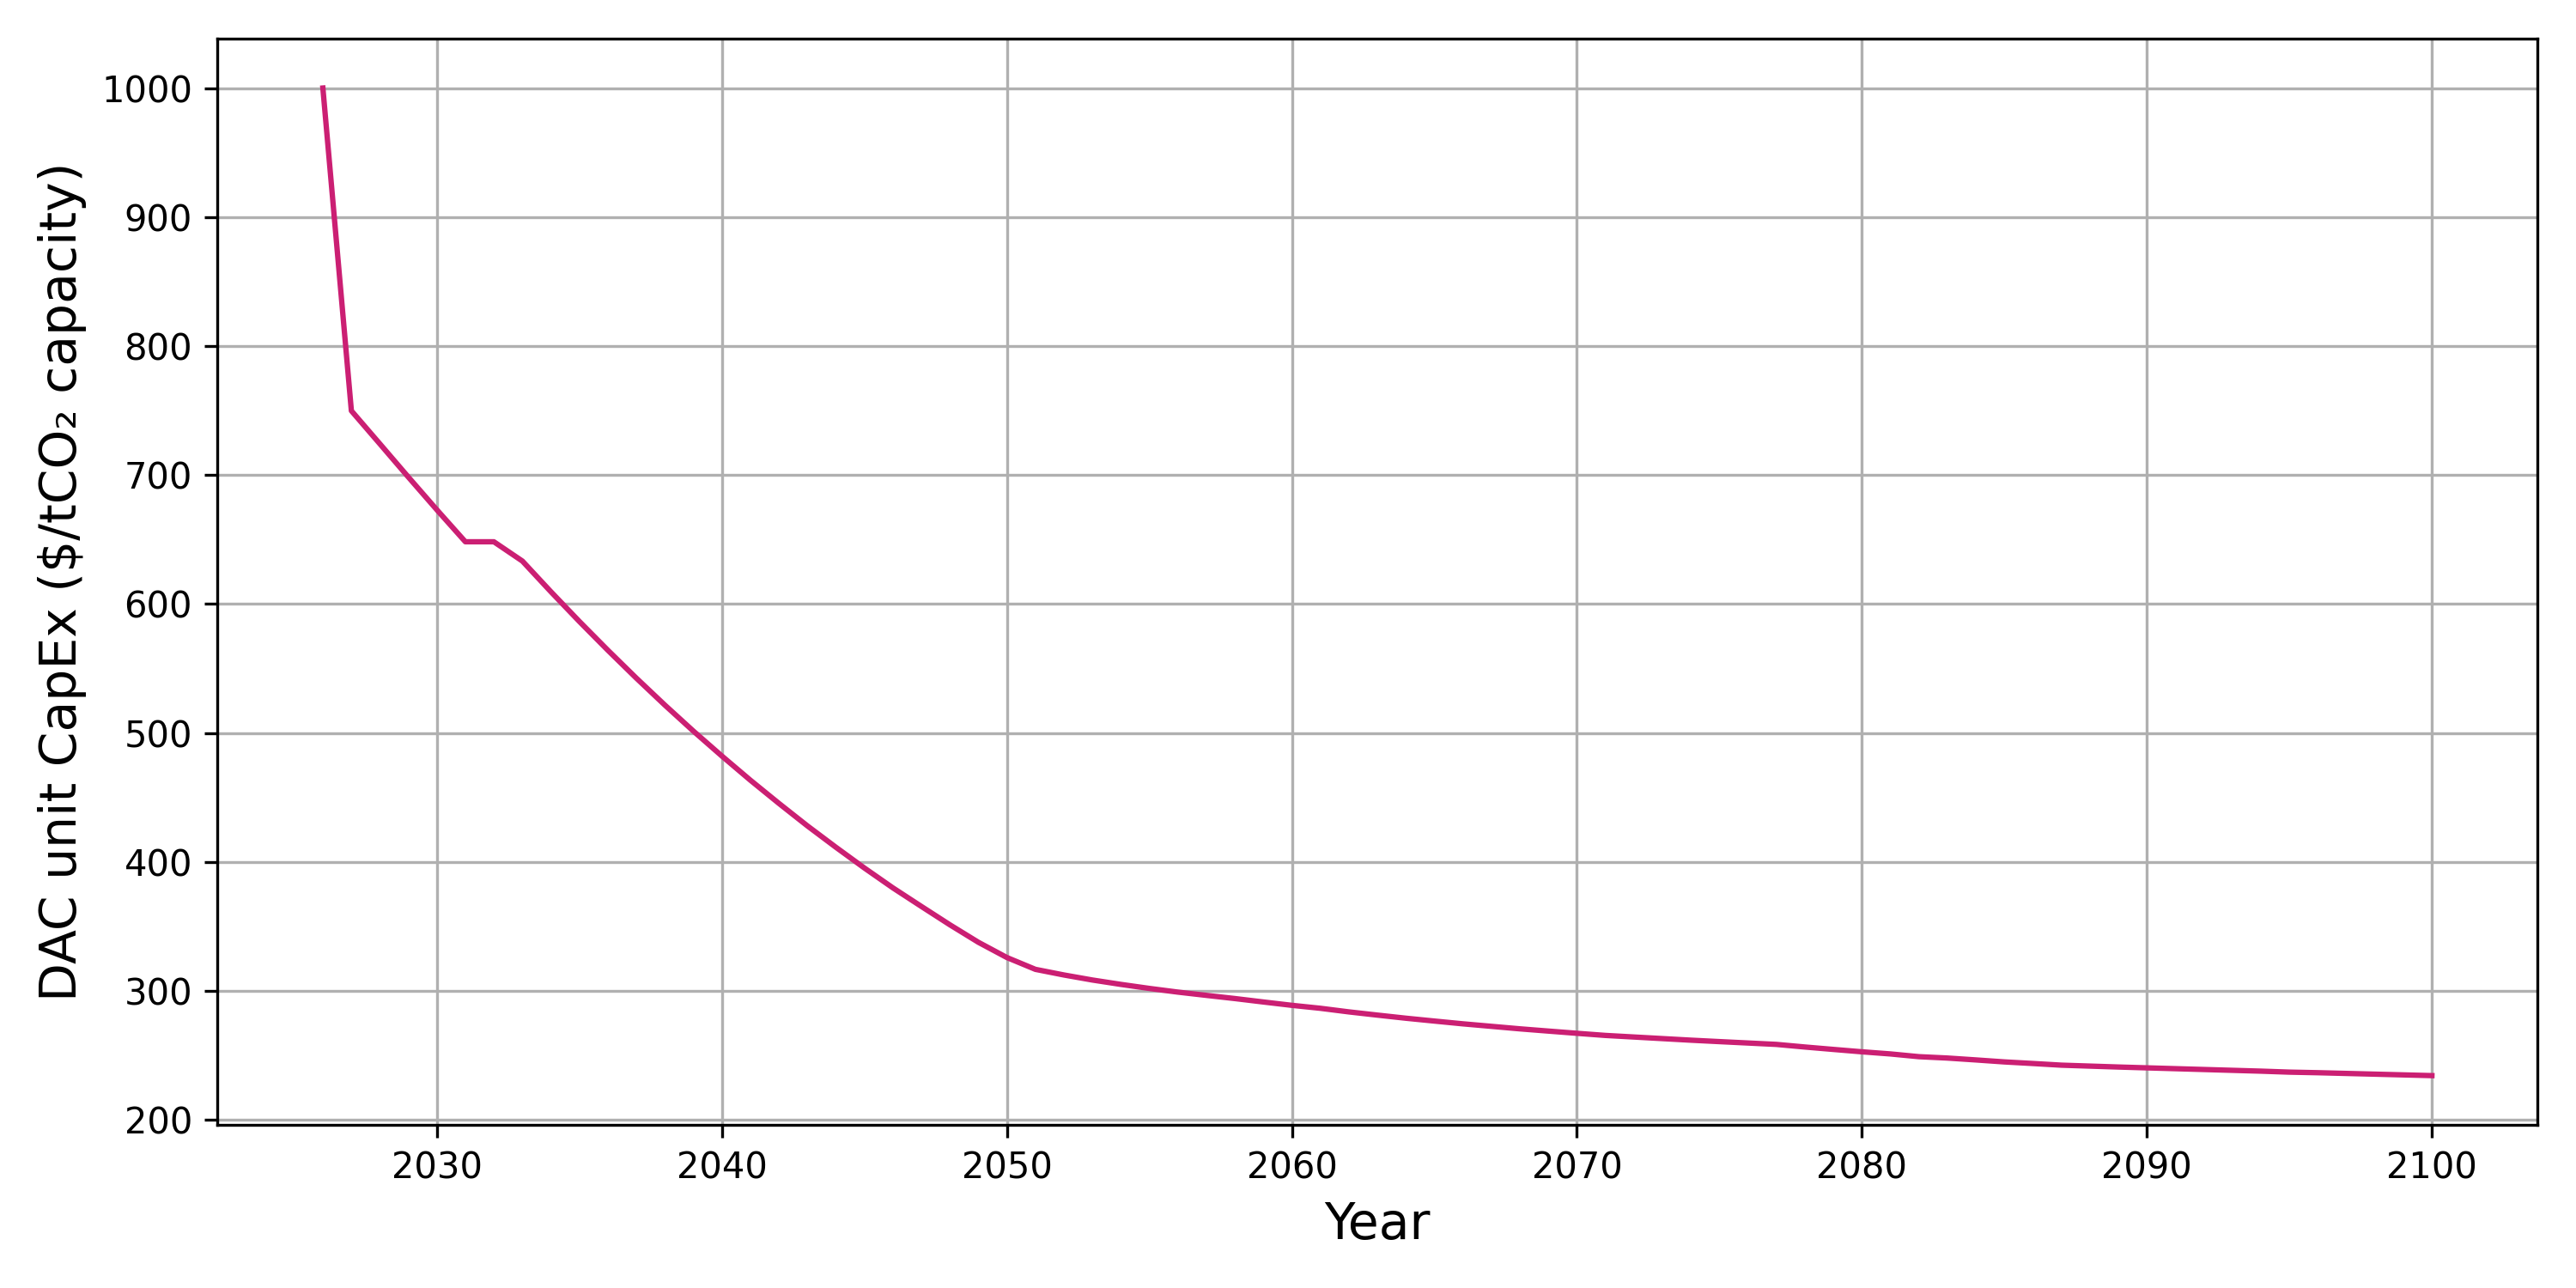
\includegraphics[width=1\linewidth]{figures/dac_capex_learning.png}
    \caption{DAC CapEx learning curve over time}
    \label{fig:dac_capex_learning}
  \end{center}
\end{figure}